\ifx\wholebook\relax \else
% ------------------------

\documentclass[b5paper]{ctexart}
\usepackage[nomarginpar
  %, margin=.5in
]{geometry}

\addtolength{\oddsidemargin}{-0.05in}
\addtolength{\evensidemargin}{-0.05in}
\addtolength{\textwidth}{0.1in}

\usepackage[cn]{../../../prelude}

\setcounter{page}{1}

\begin{document}

\title{AVL树——证明和删除算法}

\author{刘新宇
\thanks{{\bfseries 刘新宇} \newline
  Email: liuxinyu95@gmail.com \newline}
  }

\maketitle
\fi

\markboth{AVL树——证明和删除算法}{基本算法}

\ifx\wholebook\relax
\chapter{AVL树——证明和删除算法}
\numberwithin{Exercise}{chapter}
\fi

\section{插入后的高度变化}

向AVL树插入元素后,高度变化存在四种情况:

\be
\begin{array}{rcl}
  \Delta H & = & |T'| - |T| \\
           & = & 1 + max(|r'|, |l'|) - (1 + max(|r|, |l|)) \\
           & = & max(|r'|, |l'|) - max(|r|, |l|) \\
           & = & \begin{cases}
\delta \geq 0, \delta' \geq 0: & \Delta r \\
\delta \leq 0, \delta' \geq 0: & \delta + \Delta r \\
\delta \geq 0, \delta' \leq 0: & \Delta l - \delta \\
otherwise: & \Delta l
\end{cases}
\end{array}
\ee

\begin{proof}
一次插入不可能同时增加左右分支的高度。平衡因子等于右子树的高度减去左子树的高度。根据其前后变化,共有四种情况:

\begin{enumerate}
\item 如果$\delta \geq 0$并且$\delta' \geq 0$,在插入前后,右子树的高度都不小于左子树的高度。高度的增加全部“贡献”自右子树的变化$\Delta r$;

\item 如果$\delta \leq 0$,在插入前左子树的高度不小于右子树,但是插入后$\delta' \geq 0$,说明右子树的高度由于插入增加了,而左子树保持不变($|l'|=|l|$)。所以高度的增加为:

\[
\begin{array}{rll}
\Delta H & = max(|r'|, |l'|) - max (|r|, |l|) & \{\delta \leq 0\ \text{且}\ \delta' \geq 0 \}\\
         & = |r'|-|l| & \{|l|=|l'|\}\\
         & = |r|+\Delta r - |l| & \\
         & = \delta + \Delta r & \\
\end{array}
\]

\item 如果$\delta \geq 0$且$\delta' \leq 0$,和情况二类似,我们有:

\[
\begin{array}{rll}
\Delta H & = max(|r'|, |l'|) - max (|r|, |l|) & \{\delta \geq 0\ \text{且}\ \delta' \leq 0 \}\\
         & = |l'|-|r| & \\
         & = |l| + \Delta l - |r| & \\
         & = \Delta l - \delta & \\
\end{array}
\]

\item 否则$\delta$和$\delta'$都不大于0,说明插入前后左子树的高度都不小于右子树。高度的增加全部“贡献”自左子树的变化$\Delta l$。
\end{enumerate}

\end{proof}

\section{插入后平衡调整算法的证明}

如图\ref{fig:avl-insert-fix}所示,所有需要修复平衡的4种情况中,平衡因子都是-2或2。调整后,平衡因子恢复为0。左右子树具有相同的高度。

\begin{figure}[htbp]
   \begin{center}
     \setlength{\unitlength}{1cm}
     \begin{picture}(15, 15)
        % arrows
        \put(4.5, 9.5){\vector(1, -1){1}}
        \put(4.5, 5){\vector(1, 1){1}}
        \put(10, 9.5){\vector(-1, -1){1}}
        \put(10, 5){\vector(-1, 1){1}}
        % delta values
        \put(5, 13){$\delta(z) = -2$}
        \put(2.5, 12){$\delta(y) = -1$}
        \put(10, 13){$\delta(x) = 2$}
        \put(11.5, 11.5){$\delta(y) = 1$}
        \put(1.5, 5.5){$\delta(z) = -2$}
        \put(3.5, 4){$\delta(x) = 1$}
        \put(12, 5.5){$\delta(x) = 2$}
        \put(10.5, 4){$\delta(z) = -1$}
        \put(7.5, 10){$\delta'(y) = 0$}
        % graphics
    	\put(0, 7){\includegraphics[scale=0.5]{../../../datastruct/tree/AVL-tree/img/avl-insert-ll.ps}}
        \put(0, 0){\includegraphics[scale=0.5]{../../../datastruct/tree/AVL-tree/img/avl-insert-lr.ps}}
        \put(7, 7){\includegraphics[scale=0.5]{../../../datastruct/tree/AVL-tree/img/avl-insert-rr.ps}}
        \put(8.5, 0){\includegraphics[scale=0.5]{../../../datastruct/tree/AVL-tree/img/avl-insert-rl.ps}}
        \put(2, 5){\includegraphics[scale=0.5]{../../../datastruct/tree/AVL-tree/img/avl-insert-fixed.ps}}
      \end{picture}
     \caption{插入后需要恢复平衡的4种情况} \label{fig:avl-insert-fix-appendix}
  \end{center}
\end{figure}

这4种情况分别是:左-左偏、右-右偏、右-左偏、左-右偏。记修复前的平衡因子分别为$\delta(x)$、$\delta(y)$、$\delta(z)$,修复后的平衡因子分别为$\delta'(x)$、$\delta'(y)$、$\delta'(z)$。

我们接下来将证明,经过调整后,所有4种情况的平衡因子都变成$\delta(y)=0$。并且将给出调整后$\delta'(x)$和$\delta'(z)$的结果。

\subsubsection*{左-左偏(Left-left lean)的情况}

由于$x$子分支在调整前后的结构维持不变,因此可以立即得到等式:$\delta'(x) = \delta(x)$。

因为$\delta(y) = -1$且$\delta(z) = -2$,所以:

\be
  \begin{array}{l}
  \delta(y) = |C| - |x| = -1 \Rightarrow |C| = |x| - 1 \\
  \delta(z) = |D| - |y| = -2 \Rightarrow |D| = |y| - 2
  \end{array}
  \label{eq:ll-cd}
\ee

调整平衡后:

\be
  \begin{array}{rll}
  \delta'(z) & = |D| - |C| & \{ \text{根据式} (\ref{eq:ll-cd}) \}\\
             & = |y| - 2 - (|x| - 1) & \\
             & = |y| - |x| - 1 & \{  x \text{是} y \text{的子节点} \Rightarrow |y|-|x| = 1\} \\
             & = 0 &
  \end{array}
  \label{eq:ll-delta-z}
\ee

对于$\delta'(y)$,调整平衡后我们有如下结果:

\be
  \begin{array}{rll}
  \delta'(y) & = |z| - |x| & \\
             & = 1 + max(|C|, |D|) - |x| & \{ \text{根据式(\ref{eq:ll-delta-z}),我们有} |C| = |D|\} \\
             & = 1 + |C| - |x| & \{ \text{根据式(\ref{eq:ll-cd})}\} \\
             & = 1 + |x| - 1 - |x| & \\
             & = 0 &
  \end{array}
\ee

汇总上述结果,对于左-左偏的情况,新的平衡因子如下:

\be
  \begin{array}{l}
  \delta'(x) = \delta(x) \\
  \delta'(y) = 0 \\
  \delta'(z) = 0
  \end{array}
\ee

\subsubsection*{右-右偏(Right-right lean)的情况}

因为右-右偏和左-左偏对称,易知新的平衡因子结果如下:

\be
  \begin{array}{l}
  \delta'(x) = 0 \\
  \delta'(y) = 0 \\
  \delta'(z) = \delta(z)
  \end{array}
  \label{eq:rr-result}
\ee

\subsubsection*{右-左偏(Right-left lean)的情况}

首先考虑$\delta'(x)$。调整平衡后,我们有:

\be
  \delta'(x) = |B| - |A|
  \label{eq:rl-dx}
\ee

调整平衡前,如果我们计算$z$的高度,有如下的结果:

\be
  \begin{array}{rll}
  |z| & = 1 + max(|y|, |D|) &  \{ \delta(z) = -1 \Rightarrow |y| > |D|\} \\
      & = 1 + |y| & \\
      & = 2 + max(|B|, |C|)
  \end{array}
  \label{eq:rl-z}
\ee

因为$\delta(x) = 2$,所以可以推出:

\be
  \begin{array}{rll}
  \delta(x) = 2 & \Rightarrow |z| - |A| = 2 & \{ \text{根据式(\ref{eq:rl-z})} \}\\
                & \Rightarrow 2 + max(|B|, |C|) - |A| = 2 & \\
                & \Rightarrow max(|B|, |C|) - |A| = 0 &
  \end{array}
  \label{eq:rl-ca}
\ee

如果$\delta(y) = 1$,也就是$|C| - |B| = 1$,则有下面的关系:

\be
  max(|B|, |C|)= |C| = |B|+1
\ee

将其代入式(\ref{eq:rl-ca})得到:

\be
  \begin{array}{ll}
  |B|+1-|A| = 0 \Rightarrow |B|-|A|= -1 & \{ \text{根据式(\ref{eq:rl-dx}) } \} \\
  \Rightarrow \delta'(x) = -1 &
  \end{array}
\ee

反之,如果$\delta(y) \neq 1$,则有$max(|B|, |C|) = |B|$,将其代入式(\ref{eq:rl-ca})得到:

\be
  \begin{array}{ll}
  |B| - |A| = 0  & \{ \text{根据式(\ref{eq:rl-dx})} \} \\
  \Rightarrow \delta'(x) = 0 &
  \end{array}
\ee

合并上述两种子情况,我们可以得到$\delta'(x)$和$\delta(y)$的关系:

\be
\delta'(x) = \left \{
  \begin{array}
  {r@{\quad:\quad}l}
  -1 & \delta(y) = 1 \\
  0 & otherwise
  \end{array}
\right.
\label{eq:rl-dx-dy}
\ee

对于$\delta'(z)$,根据定义,它等于:

\be
  \begin{array}{rll}
    \delta'(z) & = |D| - |C| & \{ \delta(z) = -1 = |D| - |y| \} \\
               & = |y| - |C| - 1 & \{ |y| = 1 + max(|B|, |C|) \} \\
               & = max(|B|, |C|) - |C|
  \end{array}
  \label{eq:rl-dz}
\ee

如果$\delta(y) = -1$,则有$|C| - |B| = -1$,所以$max(|B|, |C|) = |B| = |C| + 1$。将其代入式(\ref{eq:rl-dz})中,我们有:$\delta'(z) = 1$。

反之,如果$\delta(y) \neq -1$,则$max(|B|, |C|) = |C|$,我们有$\delta'(z)=0$。

合并上述两种子情况,$\delta'(z)$和$\delta(y)$的关系如下:

\be
\delta'(z) = \left \{
  \begin{array}
  {r@{\quad:\quad}l}
  1 & \delta(y) = -1 \\
  0 & otherwise
  \end{array}
  \right.
  \label{eq:rl-dz-dy}
\ee

最后,对于$\delta'(y)$,我们可以推导出下面的关系:

\be
  \begin{array}{rl}
  \delta'(y) & = |z| - |x| \\
             & = max(|C|, |D|) - max(|A|, |B|)
  \end{array}
  \label{eq:rl-dy}
\ee

这里又分为3种子情况:
\begin{itemize}

\item 若$\delta(y)=0$,说明$|B|=|C|$,根据式(\ref{eq:rl-dx-dy})和式(\ref{eq:rl-dz-dy}),我们有:$\delta'(x)=0 \Rightarrow |A| = |B|$以及$\delta'(z)=0 \Rightarrow |C|=|D|$。因此$\delta'(y)=0$。

\item 若$\delta(y)=1$,根据式(\ref{eq:rl-dz-dy}),我们有$\delta'(z)=0 \Rightarrow |C| = |D|$。

\[
  \begin{array}{rll}
  \delta'(y) & = max(|C|, |D|) - max(|A|, |B|) & \{|C|=|D|\} \\
             & = |C| - max(|A|, |B|) & \{\text{根据式(\ref{eq:rl-dx-dy}): $\delta'(x)=-1 \Rightarrow |B|-|A|=-1$} \} \\
             & = |C| - (|B| + 1) & \{ \delta(y) = 1 \Rightarrow |C|-|B|=1\} \\
             & = 0
  \end{array}
\]

\item 若$\delta(y)=-1$,根据式(\ref{eq:rl-dx-dy}),我们有$\delta'(x)=0 \Rightarrow |A|=|B|$。

\[
  \begin{array}{rll}
  \delta'(y) & = max(|C|, |D|) - max(|A|, |B|) & \{|A|=|B|\} \\
             & = max(|C|, |D|) - |B| & \{ \text{根据式(\ref{eq:rl-dz-dy}): $|D|-|C|=1$} \} \\
             & = |C| + 1 - |B| & \{  \delta(y) = -1 \Rightarrow |C|-|B|=-1\} \\
             & = 0
  \end{array}
\]

\end{itemize}

全部三种情况的结果都是$\delta'(y)=0$。

将上述结果归纳起来,可以得到新的平衡因子如下:

\be
  \begin{array}{l}
  \delta'(x) = \left \{
    \begin{array}
    {r@{\quad:\quad}l}
    -1 & \delta(y) = 1 \\
    0 & otherwise
    \end{array}
    \right. \\
  \delta'(y) = 0 \\
  \delta'(z) = \left \{
    \begin{array}
    {r@{\quad:\quad}l}
    1 & \delta(y) = -1 \\
    0 & otherwise
    \end{array}
    \right.
  \end{array}
  \label{eq:rl-result}
\ee

\subsubsection*{左-右偏(Left-right lean)的情况}

左-右偏的情况和右-左偏的情况对称。使用类似的推导,我们可以得到和式(\ref{eq:rl-result})完全相同的结果。

\section{删除算法}

删除后会引起子树高度的变化。如果平衡因子因此超出了$[-1, 1]$的范围,就需要修复以维持AVL树的性质。

\subsection{函数式删除算法}

我们可以复用大部分的二叉搜索树删除算法,然后检查平衡因子并进行修复。和插入算法类似,删除的结果为一对值
$(T', \Delta H)$,其中$T'$是删除后的新树、$\Delta H$是高度的减少量。令函数$first(pair)$返回一对
值中的前一个分量。我们可以将删除算法定义如下:

\be
delete(T, k) = first(del(T, k))
\ee

其中

\be
del(T, k) = \left \{
  \begin{array}
  {r@{\quad:\quad}l}
  (\phi, 0) & T = \phi \\
  tree(del(T_l, k), k', (T_r, 0), \Delta) & k < k' \\
  tree((T_l, 0), k', del(T_r, k), \Delta) & k > k' \\
  (T_r, -1) & k = k', T_l = \phi \\
  (T_l, -1) & k = k', T_r = \phi \\
  tree((T_l, 0), k'', del(T_r, k''), \Delta) & otherwise, k'' = min(T_r)
  \end{array}
\right.
\label{eq:avl-del}
\ee

如果树为空,删除的结果也为空;否则,我们比较节点的key和待删除的值,并沿着子树递归地进行查找和删除。
如果待删除的节点含有的非空子树少于两棵,可以将其直接切下。否则,我们用右子树中的最小值替换节点的key,
然后将最小值节点切下。

我们可以复用定义好的$tree()$函数和$\Delta H$的结果。和插入算法相比,需要处理两种删除中特有的
额外情况。

\begin{figure}[htbp]
  \centering
  \subcaptionbox{AVL树删除后需要修复的情况A}{
    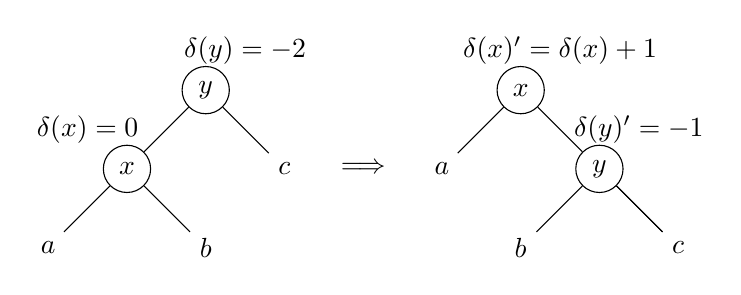
\begin{tikzpicture}[scale=1,
        trnode/.style={circle, draw, inner sep= 0pt, minimum size = .6cm}
      ]
      % left side
      \node[trnode] at (0, 0) (y) {$y$};
      \node[trnode] at (-1, -1) (x) {$x$};
      \draw (1, -1) node (c) {$c$};
      \draw (-2, -2) node (a) {$a$};
      \draw (0, -2) node (b) {$b$};
      % edges
      \draw (y) -- (x) -- (a);
      \draw (y) -- (c);
      \draw (x) -- (b);
      % labels
      \draw (0.5, 0.5) node{$\delta(y) = -2$};
      \draw (-1.5, -0.5) node{$\delta(x) = 0$};

      % right side
      \node[trnode] at (4, 0) (x1) {$x$};
      \draw (3, -1) node (a1) {$a$};
      \node[trnode] at (5, -1) (y1) {$y$};
      \draw (4, -2) node (b1) {$b$};
      \draw (6, -2) node (c1) {$c$};
      % edges
      \draw (x1) -- (y1) -- (c1);
      \draw (x1) -- (a1);
      \draw (y1) -- (b1);
      \draw (y1) -- (c1);
      % labels
      \draw (4.5, 0.5) node{$\delta(x)' = \delta(x) + 1$};
      \draw (5.5, -0.5) node{$\delta(y)' = -1$};

      \draw (2, -1) node{$\Longrightarrow$};
  \end{tikzpicture}} \\
  \subcaptionbox{AVL树删除后需要修复的情况B}{
    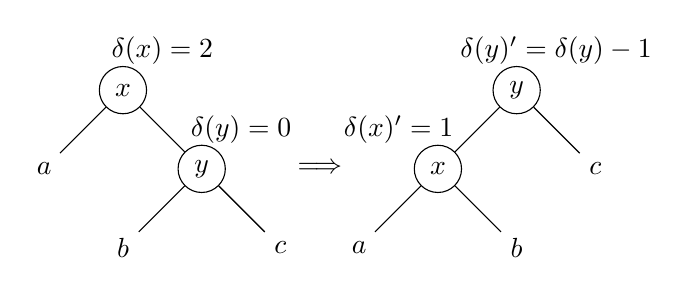
\begin{tikzpicture}[scale=1,
        trnode/.style={circle, draw, inner sep= 0pt, minimum size = .6cm}
      ]
      % left side
      \node[trnode] at (0, 0) (x) {$x$};
      \draw (-1, -1) node (a) {$a$};
      \node[trnode] at (1, -1) (y) {$y$};
      \draw (0, -2) node (b) {$b$};
      \draw (2, -2) node (c) {$c$};
      % edges
      \draw (x) -- (y) -- (c);
      \draw (x) -- (a);
      \draw (y) -- (b);
      \draw (y) -- (c);
      % labels
      \draw (0.5, 0.5) node{$\delta(x) = 2$};
      \draw (1.5, -0.5) node{$\delta(y) = 0$};

      % right side
      \node[trnode] at (5, 0) (y1) {$y$};
      \node[trnode] at (4, -1) (x1) {$x$};
      \draw (6, -1) node (c1) {$c$};
      \draw (3, -2) node (a1) {$a$};
      \draw (5, -2) node (b1) {$b$};
      % edges
      \draw (y1) -- (x1) -- (a1);
      \draw (y1) -- (c1);
      \draw (x1) -- (b1);
      % labels
      \draw (5.5, 0.5) node{$\delta(y)' = \delta(y) - 1$};
      \draw (3.5, -0.5) node{$\delta(x)' = 1$};


      \draw (2.5, -1) node{$\Longrightarrow$};
  \end{tikzpicture}}
  \caption{AVL树在删除后需要修复的两种情况} \label{fig:avl-del-fixing}
\end{figure}

如图\ref{fig:avl-del-fixing}所示,两种情况都可以通过一次树的旋转操作来修复。我们可以用模式匹配来概括这种结构上的变化。

\be
balance(T, \Delta H) = \left \{
  \begin{array}
  {r@{\quad:\quad}l}
  ... \\
  (A, x, (B, y, C, -1), \delta(x) + 1, \Delta H) & T = ((A, x, B \delta(x)), y, C, -2, \Delta H) \\
  ((A, x, B 1), y, C, \delta(y) - 1, \Delta H) & T = (A, x, (B, y, C \delta(y)), 2, \Delta H) \\
  ...
  \end{array}
\right.
\ee

下面的Haskell例子程序实现了这种AVL树的删除算法。

\lstset{language=Haskell}
\begin{lstlisting}
delete::(Ord a) => AVLTree a -> a -> AVLTree a
delete t x = fst $ del t x where
  -- 结果为一对值(t, d),t:树、d:高度的减小值
  del Empty _ = (Empty, 0)
  del (Br l k r d) x
    | x < k = node (del l x) k (r, 0) d
    | x > k = node (l, 0) k (del r x) d
    -- x == k,删除该节点
    | isEmpty l = (r, -1)
    | isEmpty r = (l, -1)
    | otherwise = node (l, 0) k' (del r k') d where k' = min r
\end{lstlisting}

其中辅助函数\texttt{min}和二叉搜索树中的定义相同,它沿着左子树遍历到尽头。函数\texttt{isEmpty}检查给定的树是否为空。

\begin{lstlisting}
isEmpty Empty = True
isEmpty _ = False

min :: AVLTree a -> a
min (Br Empty x _ _) = x
min (Br l _ _ _) = min l
\end{lstlisting}

在函数\texttt{balance}中增加用于删除的两种情况后,总共有7种情况需要修复。

\begin{lstlisting}
balance :: (AVLTree a, Int) -> (AVLTree a, Int)
balance (Br (Br (Br a x b dx) y c (-1)) z d (-2), dH) =
        (Br (Br a x b dx) y (Br c z d 0) 0, dH-1)
balance (Br a x (Br b y (Br c z d dz)    1)    2, dH) =
        (Br (Br a x b 0) y (Br c z d dz) 0, dH-1)
balance (Br (Br a x (Br b y c dy)    1) z d (-2), dH) =
        (Br (Br a x b dx') y (Br c z d dz') 0, dH-1) where
    dx' = if dy ==  1 then -1 else 0
    dz' = if dy == -1 then  1 else 0
balance (Br a x (Br (Br b y c dy) z d (-1))    2, dH) =
        (Br (Br a x b dx') y (Br c z d dz') 0, dH-1) where
    dx' = if dy ==  1 then -1 else 0
    dz' = if dy == -1 then  1 else 0
-- 删除时需要额外处理的两种情况
balance (Br (Br a x b dx) y c (-2), dH) = (Br a x (Br b y c (-1)) (dx+1), dH)
balance (Br a x (Br b y c dy)    2, dH) = (Br (Br a x b    1) y c (dy-1), dH)
balance (t, d) = (t, d)
\end{lstlisting}

\subsection{命令式删除算法}

命令式删除算法使用树的旋转操作来恢复平衡。和插入算法相比,删除需要处理更多的情况。我们首先使用二叉搜索树
删除算法,然后再修复由于子树高度变化引起的平衡问题。删除算法的基本部分描述如下:

\begin{algorithmic}[1]
\Function{Delete}{$T, x$}
  \If{$x = $ NIL}
    \State \Return $T$
  \EndIf
  \State $p \gets$ \Call{Parent}{$x$}
  \If{\Call{Left}{$x$} = NIL}
    \State $y \gets $ \Call{Right}{$x$}
    \State replace $x$ with $y$
  \ElsIf{\Call{Right}{$x$} = NIL}
    \State $y \gets $ \Call{Left}{$x$}
    \State replace $x$ with $y$
  \Else
    \State $z \gets$ \textproc{Min}(\Call{Right}{$x$})
    \State copy key and satellite date from $z$ to $x$
    \State $p \gets$ \Call{Parent}{$z$}
    \State $y \gets$ \Call{Right}{$z$}
    \State replace $z$ with $y$
  \EndIf
  \State \Return \Call{AVL-Delete-Fix}{$T, p, y$}
\EndFunction
\end{algorithmic}

首先时特殊情况。如果待删除节点为空,树没有变化。一般情况下,我们记待删除节点的父节点为$p$,如果任一子树
为空,我们将待删除节点切下,取代为另一非空子树。否则,我们在右子树中找到最小值节点$z$,将其中的key和
数据复制到待删除节点$x$,然后将$z$切下。最后,我们调用修复函数,并传入根节点、父节点、和替换掉待删除节点的
新节点。

记父节点的平衡因子为$\delta(p)$,和删除后的新平衡因子$\delta(p)'$比较,我们会发现三种不同的情况。

\begin{itemize}
\item 情况1:$|\delta(p)| = 0$、$|\delta(p)'| = 1$。这说明,虽然删除后子树的高度降低了,但是父节点
仍然满足AVL树的性质,保持平衡。算法退出;
\item 情况2:$|\delta(p)| = 1$、$|\delta(p)'| = 0$。这说明,删除前左右子树的高度差为1,删除后原来
较高的树高度减小了1。左右子树现在高度相等。结果是父节点的高度也减小了1。我们需要继续自底向上沿着父节点
更新树的高度;
\item 情况3:$|\delta(p)| = 1$、$|\delta(p)'| = 2$。这说明删除后子树的高度差违反了AVL树的性质,
我们需要通过树的旋转操作来修复平衡。
\end{itemize}

对于情况3,大部分的修复操作和插入算法相同。但是我们需要针对图\ref{fig:avl-del-fixing}中所示
的两种特殊情况,进行额外的处理。完整的修复算法如下。

\begin{algorithmic}[1]
\Function{AVL-Delete-Fix}{$T, p, x$}
  \While{$p \neq $ NIL}
    \State $l \gets$ \Call{Left}{$p$}, $r \gets$ \Call{Right}{$p$}
    \State $\delta \gets \delta(p)$, $\delta' \gets \delta$
    \If{$x = l$}
      \State $\delta' \gets \delta' + 1$
    \Else
      \State $\delta' \gets \delta' - 1$
    \EndIf
    \If{$p$ is leaf} \Comment{$l = r =$ NIL}
      \State $\delta' \gets 0$
    \EndIf
    \If{$|\delta| = 1 \land |\delta'| = 0$}
      \State $x \gets p$
      \State $p \gets$ \Call{Parent}{$x$}
    \ElsIf{$|\delta| = 0 \land |\delta'| = 1$}
      \State \Return $T$
    \ElsIf{$|\delta| = 1 \land |\delta'| = 2$}
      \If{$\delta' = 2$}
        \If{$\delta(r) = 1$} \Comment{右-右情况}
          \State $\delta(p) \gets 0$
          \State $\delta(r) \gets 0$
          \State $p \gets r$
          \State $T \gets $ \Call{Left-Rotate}{$T, p$}
        \ElsIf {$\delta(r) = -1$} \Comment{右-左情况}
          \State $\delta_y \gets \delta($ \Call{Left}{$r$} $)$
          \If{$\delta_y = 1$}
            \State $\delta(p) \gets -1$
          \Else
            \State $\delta(p) \gets 0$
          \EndIf
          \State $\delta($ \Call{Left}{$r$} $) \gets 0$
          \If{$\delta_y = -1$}
            \State $\delta(r) \gets 1$
          \Else
            \State $\delta(r) \gets 0$
          \EndIf
        \Else \Comment{删除特有的右-右情况}
          \State $\delta(p) \gets 1$
          \State $\delta(r) \gets \delta(r) - 1$
          \State $T \gets$ \Call{Left-Rotate}{$T, p$}
          \State break \Comment{高度不再变化}
        \EndIf
      \ElsIf{$\delta' = -2$}
        \If{$\delta(l) = -1$} \Comment{左-左情况}
          \State $\delta(p) \gets 0$
          \State $\delta(l) \gets 0$
          \State $p \gets l$
          \State $T \gets $ \Call{Right-Rotate}{$T, p$}
        \ElsIf {$\delta(l) = 1$} \Comment{左-右情况}
          \State $\delta_y \gets \delta($ \Call{Right}{$l$} $)$
          \If{$\delta_y = -1$}
            \State $\delta(p) \gets 1$
          \Else
            \State $\delta(p) \gets 0$
          \EndIf
          \State $\delta($ \Call{Right}{$l$} $) \gets 0$
          \If{$\delta_y = 1$}
            \State $\delta(l) \gets -1$
          \Else
            \State $\delta(l) \gets 0$
          \EndIf
        \Else \Comment{删除特有的左-左情况}
          \State $\delta(p) \gets -1$
          \State $\delta(l) \gets \delta(l) + 1$
          \State $T \gets$ \Call{Right-Rotate}{$T, p$}
          \State break \Comment{高度不再继续变化}
        \EndIf
      \EndIf
      \Comment{高度减小,继续自底向上更新}
      \State $x \gets p$
      \State $p \gets$ \Call{Parent}{$x$}
    \EndIf
  \EndWhile
  \If{$p = $ NIL} \Comment{删除根节点}
    \State \Return $x$
  \EndIf
  \State \Return $T$
\EndFunction
\end{algorithmic}

下面的C++例子程序实现了AVL树的删除算法。

\lstset{language=C++}
\begin{lstlisting}
Node* del(Node* t, Node* x) {
    if (!x) return t;
    Node *y, *parent = x->parent;
    if (!x->left) {
        y = x->replaceWith(x->right);
    } else if (!x->right) {
        y = x->replaceWith(x->left);
    } else {
        y = min(x->right);
        x->key = y->key;
        parent = y->parent;
        x = y;
        y = y->replaceWith(y->right);
    }
    t = deleteFix(t, parent, y);
    remove(x);
    return t;
}
\end{lstlisting}

其中方法\texttt{replaceWith(tree)}用传入的子树替换掉当前节点,它返回新节点作为结果。

\begin{lstlisting}
Node* replaceWith(Node* y) {
    return replace(parent, this, y);
}
\end{lstlisting}

函数\texttt{replace(parent, x, y)}用子树\texttt{y}替换掉父节点的子树\texttt{x}。

\begin{lstlisting}
// change from: parent --> x to parent --> y
Node* replace(Node* parent, Node* x, Node* y) {
    if (!parent) {
        if (y) y->parent = nullptr;
    } else if (parent->left == x) {
        parent->setLeft(y);
    } else {
        parent->setRight(y);
    }
    if (x) x->parent = nullptr;
    return y;
}
\end{lstlisting}

函数\texttt{min(t)}递归地查找子树的最小值节点。函数\texttt{remove(tree)}用于将节点释放。

\begin{lstlisting}
Node* min(Node* t) {
    while (t && t->left) t = t->left;
    return t;
}

void remove(Node* x) {
    if (x) {
        x->parent = x->left = x->right = nullptr;
        delete x;
    }
}
\end{lstlisting}

修复函数的实现如下。

\begin{lstlisting}
Node* deleteFix(Node* t, Node* parent, Node* x) {
    int d1, d2, dy;
    Node *p, *l, *r;
    while (parent) {
        d2 = d1 = parent->delta;
        d2 += (x == parent->left ? 1 : -1);
        if (isLeaf(parent)) d2 = 0;
        parent->delta = d2;
        p = parent;
        l = parent->left;
        r = parent->right;
        if (abs(d1) == 1 && abs(d2) == 0) {
            x = parent;
            parent = x->parent;
        } else if (abs(d1) == 0 && abs(d2) == 1) {
            return t;
        } else if (abs(d1) == 1 && abs(d2) == 2) {
            if (d2 == 2) {
                if (r->delta == 1) {  // 右-右情况
                    p->delta = r->delta = 0;
                    parent = r;
                    t = leftRotate(t, p);
                } else if (r->delta == -1) { // 右-左情况
                    dy = r->left->delta;
                    p->delta = dy == 1 ? -1 : 0;
                    r->left->delta = 0;
                    r->delta = dy == -1 ? 1 : 0;
                    parent = r->left;
                    t = rightRotate(t, r);
                    t = leftRotate(t, p);
                } else { // 删除特有的右-右情况
                    p->delta = 1;
                    r->delta--;
                    t = leftRotate(t, p);
                    break; // 高度不再继续变化
                }
            } else if (d2 == -2) {
                if (l->delta == -1) { // 左-左情况
                    p->delta = l->delta = 0;
                    parent = l;
                    t = rightRotate(t, p);
                } else if (l->delta == 1) { // 左-右情况
                    dy = l->right->delta;
                    l->delta = dy == 1 ? -1 : 0;
                    l->right->delta = 0;
                    p->delta = dy == -1 ? 1 : 0;
                    parent = l->right;
                    t = leftRotate(t, l);
                    t = rightRotate(t, p);
                } else { // 删除特有的左-左情况
                    p->delta = -1;
                    l->delta++;
                    t = rightRotate(t, p);
                    break; // 高度不再继续变化
                }
            }
            // 以上修复会造成高度减小,需要继续自底向上更新
            x = parent;
            parent = x->parent;
        } else {
            printf("shouldn't be here, d1 = %d, d2 = %d", d1, d2);
            assert(false);
        }
    }
    if (!parent) return x; // 删除根节点
    return t;
}
\end{lstlisting}

\begin{Exercise}
比较AVL树的命令式删除和插入算法,将共同的部分抽出,实现一个通用的AVL树修复算法。
\end{Exercise}

\ifx\wholebook\relax \else
%% \begin{thebibliography}{99}

%% \bibitem{CLRS}
%% Thomas H. Cormen, Charles E. Leiserson, Ronald L. Rivest and Clifford Stein.
%% ``Introduction to Algorithms, Second Edition''. ISBN:0262032937. The MIT Press. 2001

%% \end{thebibliography}

\end{document}
\fi
